\section{Historical background}

Baltic scientists in their research \cite{slavic-procent} worked out a model of Slavic lexical identity. In the picture, you can see the percentage of common lexicon provided by connections between different Slavic languages.

There are three Slavic linguistic and ethnic branches - East Slavic (Russian, Belorussian, Ukrainian and Rusyn), West Slavic (Czech, Slovak, Polish, Kashubian, Silesian, Upper-Sorbian, Lower-Sorbian) and South Slavic (Slovenian, Serbian, Croatian, Macedonian and Bulgarian).

This division goes back into history. Different communication events with other nations, geographical position, territorial pecularity - everything affected Slavic people that became nations that now exist. It is supposed to have three initial tribes of Slavs: Venedes (the ancestors of West Slavs), Antes (the ancestors of East Slavs) and Sklavins (the ancestors of South Slavs). It is controversial, but a viable and a rather popular model within Slavic community.

\begin{figure}
	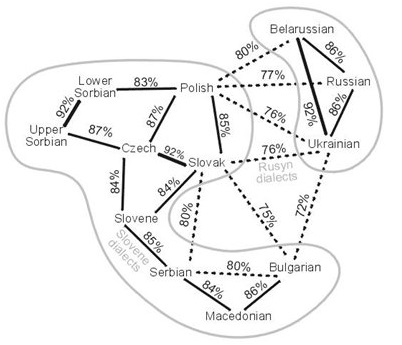
\includegraphics[width=\linewidth]{./sources/percents.jpg}
	\caption{Lexicon connections in Slavic languages}
	\label{fig:percent}
\end{figure}

Nevertheless, Slavs started to separate from each other in the seventh century. South Slavs came to Balkan peninsula and assimulated the Illyrian and Turkic peoples that lived there already. Thus, we see how Croatians and Bulgars appeared. The confrontation of Slavs and Germans lead to West Slavic peoples' appearance. Spreading to the East and confrontation with Finno-Ugric and Turkic peoples poured out into the appearance of East Slavic nations.